\subsection{Maximierung des Zuwachses der Klassifizierungsgenauigkeit}
Scikit-Learn bietet viele Parameter an, um den Teilungsprozess bei der Konstruktion zu steuern. Einer dieser Parameter ist \texttt{min\_samples\_leaf}, d. h. die minimale Anzahl an Einträgen der Trainingsmenge
in einem Blatt. Dieser steuert die minimale Anzahl an Einträgen die in einem Kindknoten enthalten sein müssen, nachdem ein Knoten geteilt wurde. Standardmäßig ist der Wert 1. Dadurch entsteht ein sehr fein granularer
Entscheidungsbaum, der viele Blätter mit nur einem Eintrag hat. Das heißt, es wurden Teilungen durchgeführt, die nur zwei Einträge unterteilt haben. Der Zuwachs der Klassifizierungsgenauigkeit ist durch diese
Teilungen sehr gering. Eine Erhöhung in der Blattgröße verspricht, dass Entscheidungsbäume gefunden werden können, die zwar tiefer sind, aber dafür eine bessere Klassifizierungsgenauigkeit pro Vergleich erzielen.
Der Baum kann tiefer werden, da die Grenze des Programmspeichers noch nicht erreicht wurde.
\newline
\newline
Abbildung \ref{fig:msl} zeigt, wie sich der Parameter auf verschieden große Trainingsmengen auswirkt. Betrachtet wird eine Maximalhöhe von 16. Besonders bei großen Trainingsmengen (Abbildung \ref{subfig:msl_big})
kann die Programmgröße mit einer Blattgröße von 8 signifkant sinken, ohne die maximale Baumhöhe zu beeinflussen. Bei kleinen Trainingsmengen (Abbildung \ref{subfig:msl_small}) reduziert bereits bei kleinen Blattgrößen
sich die Programmgröße ebenfalls signifikant. Allerdings wird die maximale Baumhöhe beeinflusst. Besonders bei großen Trainingsmengen wirkt sich der Parameter stärker auf die Programmgröße aus.
Vermutlich, da die Anzahl der Blätter sich signifikant erhöht, je tiefer der Baum ist.
\subfigbox{
\subfigure[Trainingsmengengröße: 1023]{\label{subfig:msl_small}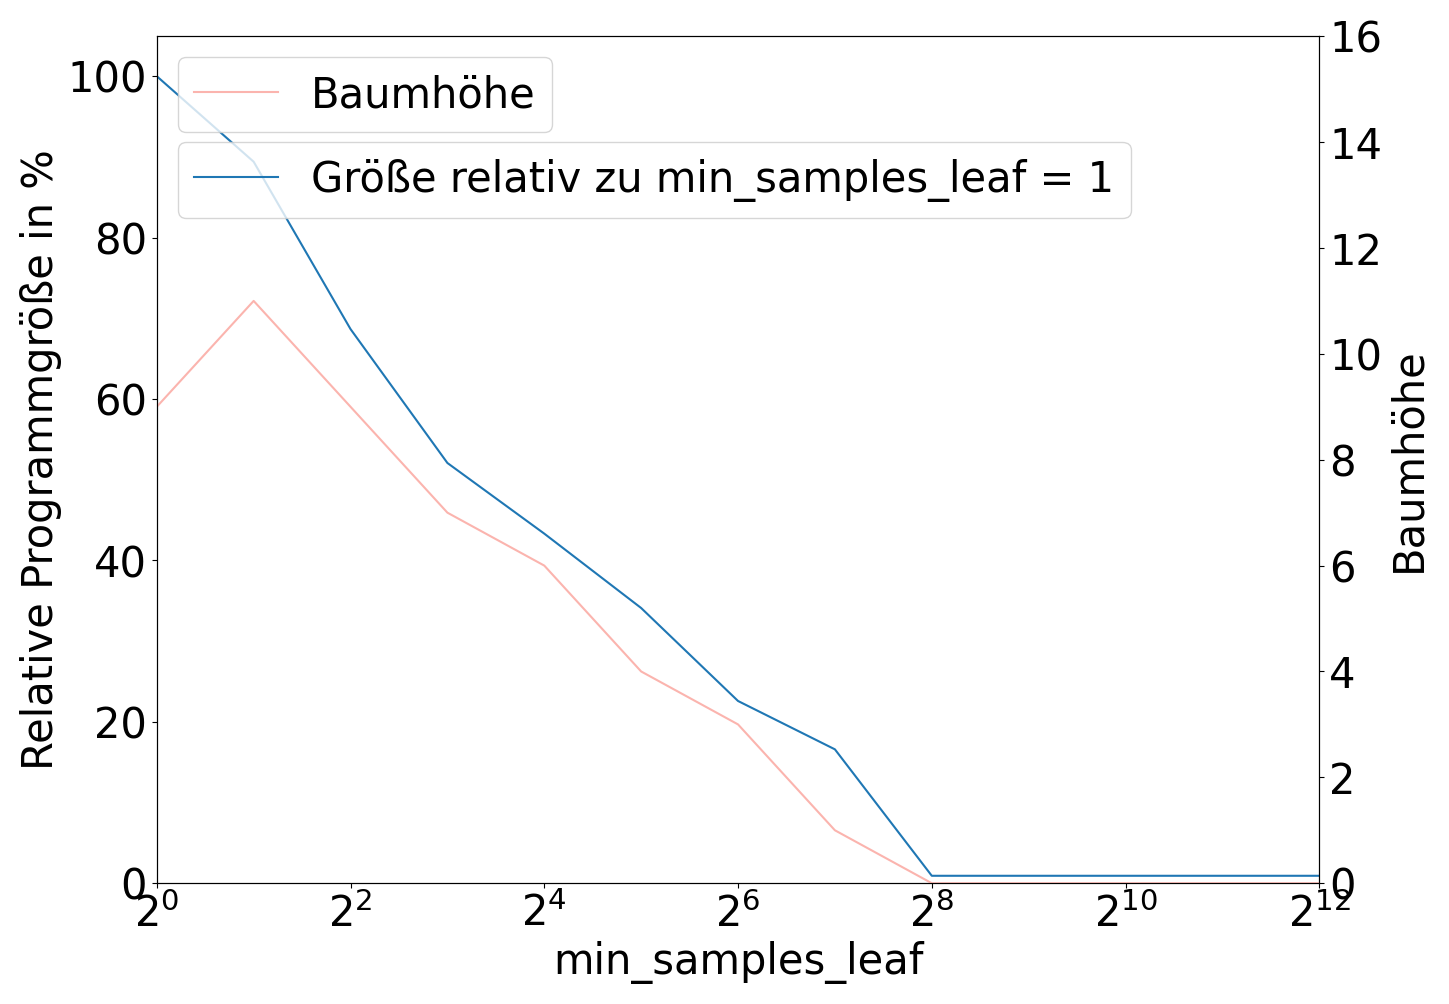
\includegraphics[width=0.48\linewidth]{images/min_samples_leaf_small.png}}\hfill%
\subfigure[Trainingsmengengröße: 7629]{\label{subfig:msl_big}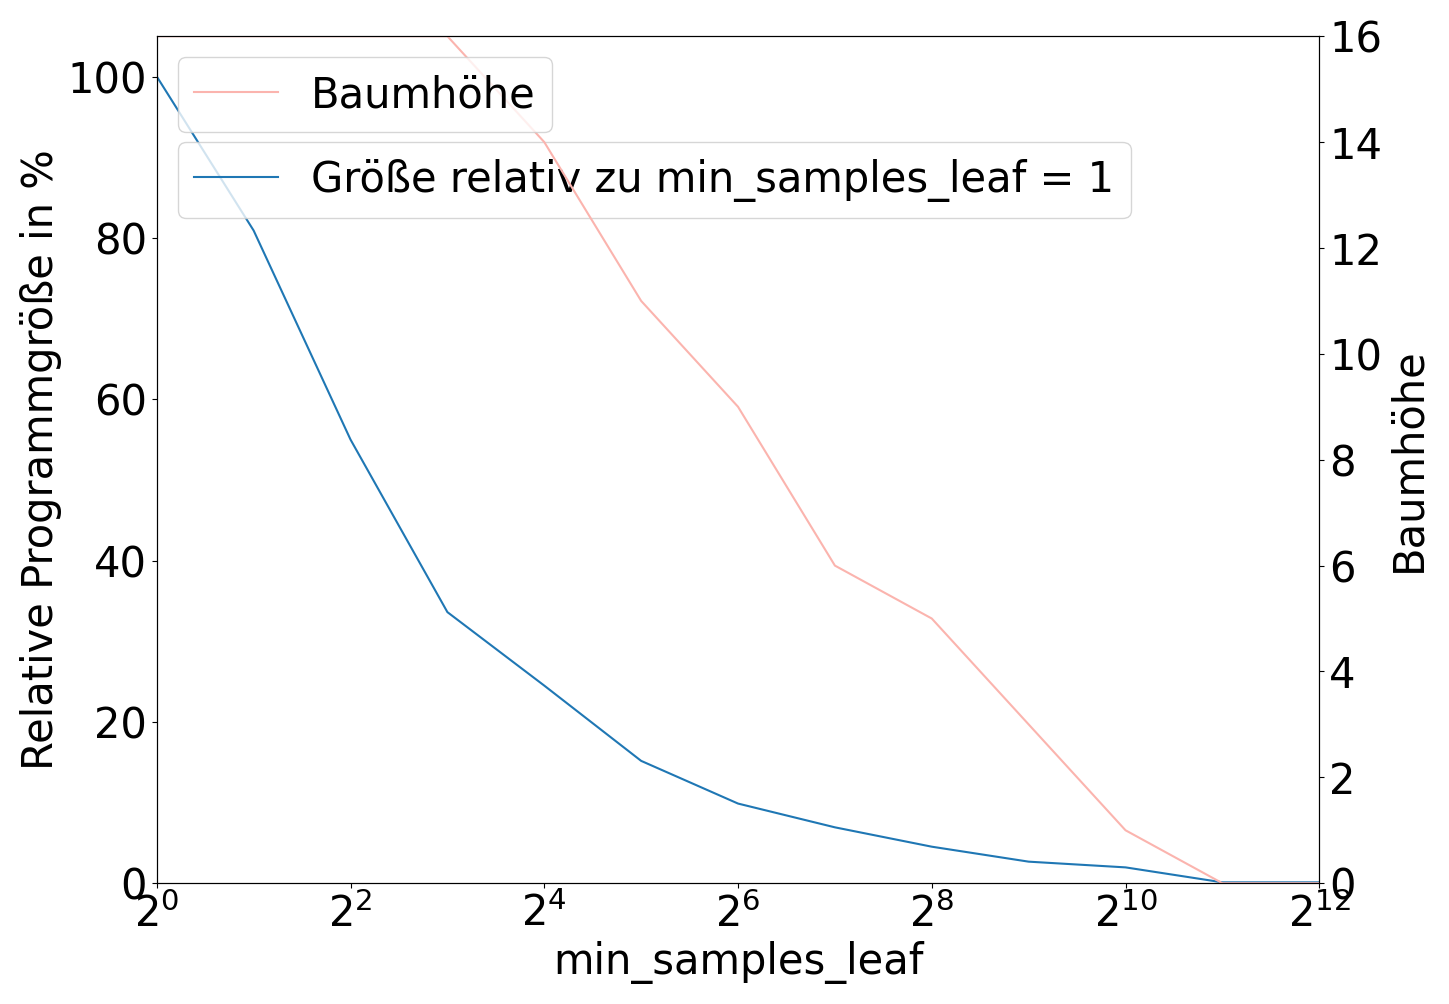
\includegraphics[width=0.48\linewidth]{images/min_samples_leaf_big.png}}%
}{Auswirkung der minimalen Blattgröße auf die Programmgröße und Baumhöhe.}{fig:msl}
\newline
\newline
Es kann nicht argumentiert werden, dass ein Wert für die Blattgröße besser ist als ein Anderer, da die Klassifizierungsgenauigkeit auf der Trainingsmenge keine Aussage über die Klassifizierungsgenauigkeit auf
der Testmenge treffen kann. Eine hohe Klassifizierungsgenauigkeit auf Trainingsmenge muss nicht umbedingt eine hohe Klassifizierungsgenauigkeit auf der Testmenge implizieren. Allerdings können so vermeintlich
höhere Entscheidungsbäume ausgewählt werden, da diese weniger Programmspeicher benötigen im Vergleich zu gleich hohen Entscheidungsbäumen mit einer geringeren Blattgröße. Dieser Parameter vergrößert folglich
den Suchraum. Bei kleinen Trainingsmengen ist eine Blattgröße über 1 nur sinnvoll, wenn der größte Entscheidungsbaum, der generiert werden kann, nicht innerhalb der Restriktionen des Programmspeichers liegt.